\usepackage{ifthen}
\usepackage{intcalc}
\usepackage{amsmath}
\usepackage{tikz}

\newcounter{tartaglia}
\newcounter{newton}
\newcounter{i}% contatore delle righe
\newcounter{j}% contatore delle colonne
\newcounter{n}% è il numero massimo di righe
\newcounter{I}% contatori di servizio
\newcounter{J}%

%creazione del comando ``cbinomiale''
\newcommand{\cbinomiale}[2]{%
	\intcalcDiv{\intcalcFac{#1}}{\intcalcMul{\intcalcFac{#2}}{\intcalcFac{\intcalcSub{#1}{#2}}}}
}

%creazione del comando ``Binomio di Newton''
\newcommand{\newton}[1]{%
	\stepcounter{newton}%
	\setcounter{i}{1}%
	\setcounter{j}{0}%
	\setcounter{n}{#1}%
		\begin{center}
		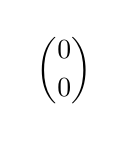
\begin{tikzpicture}[node distance=15 mm]
			\node (\thenewton_n0_0){$\displaystyle\binom{0}{0}$};
			\whiledo{\thei<\then}{%
			\setcounter{I}{\thei}%
			\addtocounter{I}{-1}%
				\whiledo{\thej<\thei}{%
					\setcounter{J}{\thei}%
					\addtocounter{J}{-1}%
						\node[below left of=\thenewton_n\theI_\thej](\thenewton_n\thei_\thej){$\displaystyle\binom{\thei}{\thej}$};
						\stepcounter{j}%
					}
				\node[below right of=\thenewton_n\theI_\theJ](\thenewton_n\thei_\thej){$\displaystyle\binom{\thei}{\thej}$};
				\stepcounter{i}%
				\setcounter{j}{0}%
			}
		\end{tikzpicture}
		\end{center}
}
	
%creazione del comando ``Triangolo di Tartaglia''
	\newcommand{\tartaglia}[2]{%
		\stepcounter{tartaglia}%
		\setcounter{i}{1}%
		\setcounter{j}{0}%
		\setcounter{n}{#1}%
			\begin{center}
			\begin{tikzpicture}[node distance=#2 mm]
				\node (\thetartaglia_t0_0){\cbinomiale{0}{0}};
				\whiledo{\thei<\then}{%
				\setcounter{I}{\thei}%
				\addtocounter{I}{-1}%
					\whiledo{\thej<\thei}{%
						\setcounter{J}{\thei}%
						\addtocounter{J}{-1}%
							\node[below left of=\thetartaglia_t\theI_\thej](\thetartaglia_t\thei_\thej){\cbinomiale{\thei}{\thej}};
							\stepcounter{j}%
						}
					\node[below right of=\thetartaglia_t\theI_\theJ](\thetartaglia_t\thei_\thej){\cbinomiale{\thei}{\thej}};
					\stepcounter{i}%
					\setcounter{j}{0}%
				}
			\end{tikzpicture}
			\end{center}
}
